\part{Генератор синтаксических анализаторов, построенный на базе \GRM{}}\label{part3}

\GRM{} предоставляет единый формат для записи контекстно-свободных грамматик и спецификаций на их основе. Если спецификация содержит дополнительную информацию, \GRM{} позволяет хранить ее в аннотациях. Как было показано выше, метаданные можно отделять от грамматики с помощью аспектов, получая несколько спецификаций из одной грамматики.

В настоящей главе мы рассмотрим генератор трансляторов \ATF{}, использующий возможности \GRM{} для решения задачи порождения кода транслятора сразу на нескольких языках программирования, причем гарантируется, что сгенерированный код не содержит ошибок типизации.

\chapter{Генераторы трансляторов}

Генератор трансляторов принимает на вход некоторую спецификацию и порождает код на некотором языке программирования, способный выполнять трансляцию текста во внутреннее представление в соответствии с правилами, указанными в спецификации.
Формат входных данных генератора мы будем называть \term{языком спецификации}, а язык программирования, код на котором генерируется --- \term{языком реализации}. Язык, синтаксис (и, возможно, семантику) которого описывает спецификация, мы будем называть \term{анализируемым языком}.

Языки спецификаций обычно основываются на атрибутных грамматиках \cite{???Knuth} в той или иной форме. В случае \ATF{} спецификация описывает схему синтаксически-управляемой трансляции \cite{???Dragon}, соответствующей \term{L-атрибутной грамматике} \cite{???}. Особенность таких грамматик состоит в том, что вне зависимости от направления анализа (нисходящий/восходящий) для вычисления атрибутов не требуется построения полного синтаксического дерева, поскольку атрибуты удается вычислять в процессе разбора. Наиболее популярные генераторы трансляторов используют именно этот подход \cite{???}.

\section{Модули анализа и генерации}\label{antlr_example}

Любой генератор можно логически разделить на два взаимодействующих модуля: \term{модуль анализа}, читающий спецификацию, проверяющий ее корректность, и преобразующий ее во внутреннее представление, и \term{модуль генерации}, непосредственно порождающий код, читая внутреннее представление.
Модулей генерации может быть несколько, поскольку для переносимости реализации анализируемого языка и повторного использования спецификаций важно иметь возможность генерировать код на разных языках реализации.

// Рис?

Для удобства программиста важно выполнение следующего требования: \emph{если модуль анализа не обнаружил в спецификации ошибок и успешно построил внутреннее представление, модуль генерации должен построить код, не содержащий ошибок}.

В современных генераторах трансляторов это требование не соблюдается, что негативно сказывается на производительности разработчика. Проиллюстрируем это на примере разработки простого языка арифметических выражений с помощью одного из наиболее широкого используемых на сегодняшний день генераторов --- \tool{ANTLR}. Грамматика этого языка (без семантических действий) приведена в \lstref{arithexp}.
\begin{lstlisting}[texcl,language=ANTLR,label=arithexp,float=htbp,caption=Спецификация \tool{ANTLR} для языка арифметических выражений]
// Лексические правила
fragment LETTER : 'a'..'z' | 'A'..'Z' | '_' ;
fragment DIGIT  : '0'..'9' ;
VAR    : LETTER (LETTER | DIGIT)* ;
INT    : DIGIT+ ;
// Синтаксические правила
expr   : term (('+' | '-') term)* ;
term   : factor ('*' factor)* ;
factor : VAR | INT | '(' expr ')' ;
\end{lstlisting}
Нотация \tool{ANTLR} очень близка к нотации \GRM{} и в пояснении, по нашему мнению, не нуждается. Пусть необходимо разработать транслятор данного языка, вычисляющий значение выражения в процессе разбора. При этом значения переменных задаются внешней средой в виде объекта класса \code{Environment}, позволяющего получить значение переменной по имени. \tool{ANTLR} генерирует синтаксический анализатор основанный на методе рекурсивного спуска, поэтому каждое синтаксическое правило можно рассматривать как функцию, принимающую параметры (наследуемые атрибуты) и возвращающую значения (синтезируемые атрибуты). Семантические действия для правил \term{expr}, \term{term} и \term{factor} будут принимать объект \code{Environment} в качестве параметра и возвращать целочисленный результат вычисления. Соответствующий код на языке \tool{Java} пишется в фигурных скобках в том месте правила, где он должен быть вызван, аналогично схеме трансляции. 

Рассмотрим следующий вариант реализации семантических действий для правила \code{factor}:
\begin{lstlisting}[language=ANTLR]
factor[Environment env] returns [int result]
	: VAR { result = env.getValue($VAR.getText()); }
	| INT { result = $INT; }
	| '(' e=expr[env] ')' { result = e; } ;
\end{lstlisting}
По этой спецификации \tool{ANTLR} успешно генерирует код, содержащий следующий строки:
\begin{lstlisting}[language=Java,escapechar={!}]
	int result = 0;
	// ...
	Token INT2=null;
	// ...
	result = INT2;
\end{lstlisting}
При попытке скомпилировать этот фрагмент компилятором \tool{Java}, мы получим сообщение об ошибке на последней строке: значение \code{INT2} типа \code{Token} не может быть присвоено переменной \code{result}, имеющей тип \code{int}. Чтобы определить, в чем причина возникновения этой ошибки, нам необходимо вернуться к спецификации и вручную сопоставить сгенерированный код с соответствующим семантическим действием. В результате мы обнаружим, что использовали саму лексему \code{\$INT} вместо соответствующего ей текста, который можно получить, вызвав метод \code{getText()}. Мы вносим исправление в спецификацию:
\begin{lstlisting}[language=ANTLR]
factor //...
	| INT { result = $INT.getText(); }
\end{lstlisting}%$
Теперь нам необходимо снова запустить \tool{ANTLR}, чтобы получить и новую версию кода на \tool{Java}, а затем скомпилировать ее. Компилятор снова выдает сообщение об ошибке: значение \code{INT2.getText()} типа \code{String} не может быть присвоено переменной \code{result}, имеющей тип \code{int}. Мы снова возвращаемся к спецификации и конвертируем строку в число:
\begin{lstlisting}[language=ANTLR]
	| INT { result = Integer.parseInt($INT.getText()); }
\end{lstlisting}%$
После еще одного цикла генерации и компиляции, мы убеждаемся, что ошибка устранена. Всего нам понадобилось трижды запустить генератор и компилятор и дважды проследить, в каком месте в спецификации содержится причина возникновения ошибки в сгенерированном коде.

\section{Подходы, реализованные в современных генераторах}

В общем виде этот процесс, реализующийся при использовании любого генератора, не соответствующего сформулированному выше требованию, можно описать с помощью цикла, показанного на \figref{cycles} (а).
\begin{figure}[htbp]
\centering
\framebox{
\begin{minipage}{.45\textwidth}
\begin{enumerate}
\setlength{\itemsep}{0pt}
		\item Изменить спецификацию.
		\item Сгенерировать код.
		\item Попытаться скомпилировать код.
		\item Получить сообщения об ошибках в терминах языка реализации.
		\item Вручную отследить причины возникновения ошибок, содержащиеся в спецификации.
		\item Перейти к пункту 1.
\end{enumerate}
\centering
(а)
\end{minipage}
}
\framebox{
\begin{minipage}{.45\textwidth}
\begin{enumerate}
\setlength{\itemsep}{0pt}
		\item Изменить спецификацию.
		\item Попытаться сгенерировать код.
		\item Получить сообщения об ошибках в терминах языка спецификации.
		\item Перейти к пункту 1.
\end{enumerate}
\vspace{82pt}
\centering
(б)
\end{minipage}
}
\caption{Процесс устранения ошибки: (а) без статических проверок, (б) с проверками}\label{cycles}
\end{figure}
Основную сложность представляет необходимость вручную определять фрагмент спецификации, вызывающий ошибку. В принципе, модуль анализа мог бы делать это автоматически, но большинство современных инструментов, таких как \tool{ANTLR} или \tool{Bison} этого не делают, ограничиваясь лишь проверкой простейших условий, таких как наличие определений для всех символов, использованных в грамматике, без выполнения которых невозможно построение внутреннего представления. Семантические действия в этих инструментах рассматриваются как текстовые строки, и их содержание не анализируется.

Существуют генераторы, помогающие программисту в решении описанной проблемы. Так система \tool{Eli} \cite{???} анализирует сообщения об ошибках, выдаваемые компилятором, и автоматически находит соответствующие места в спецификации. Этот подход имеет два недостатка: во-первых, он привязан не только к одному языку реализации (используется язык \tool{C}), но и к одной версии компилятора, поскольку формат сообщений об ошибках может меняться. Система \tool{JastAdd} \cite{???} интегрируется с компилятором \tool{Java} и осуществляет точную диагностику ошибок, однако поддержка других языков реализации при таком подходе невозможна. Другой подход реализован в генераторе \tool{SableCC} \cite{???}: язык спецификаций вообще не поддерживает семантических действий, вместо этого разработчик должен вручную написать код на языке реализации, осуществляющий обход абстрактного синтаксического дерева и вычисляющий атрибуты. Такой подход в большей степени подвержен ошибкам и требует создания большего количества однотипного неинформативного кода.

\section{Задача \ATF{}}

Задачей \ATF{} является сокращение цикла работы со спецификацией до состояния, представленного на \figref{cycles} (б), при этом поддерживается возможность генерации кода на нескольких языках реализации по одной и той же спецификации.
Такая функциональность достигается за счет того, что семантические действия пишутся на абстрактном языке, в котором модуль анализа проверяет соблюдение правил типизации, а различные модули генерации строят код на соответствующих языках реализации.

В следующих разделах мы опишем язык спецификации, соответствующую систему типов и способы конфигурации модулей генерации и интеграции с различными языками реализации.

\chapter{Язык спецификаций \ATF{}}

\ATF{} использует нотацию \GRM{} для описания лексики и грамматики языков, при этом лексические правила явным образом помечаются атрибутом \code{lexical}, а игнорируемые терминалы, например, комментарии и пробельные символы --- еще и атрибутом \code{ignore}.

Спецификация описывает L-атрибутную трансляцию, при этом, аналогично \tool{ANTLR}, каждому правилу ставится в соответствие \term{функция трансляции}, принимающая наследуемые атрибуты в качестве параметров и возвращающая синтезируемые атрибуты. Это не означает, что \ATF{} способен генерировать только нисходящие анализаторы, использующие метод рекурсивного спуска, поскольку в случае восходящего анализа L-атрибутные определения тоже можно вычислить, вводя дополнительные продукции\footnote{Это делается автоматически в соответствующем модуле генерации.} \cite{???}. Тем не менее, о конструкциях, используемых в \ATF{}, удобнее всего думать в терминах рекурсивного спуска.

Телом функции трансляции, соответствующей правилу, является спецификация семантических действий, относящихся к различным позициям внутри правила, а также значения аргументов, передаваемых функциям трансляции, соответствующим символам, входящим в правые части продукций данного правила. В следующих подразделах мы опишем основные конструкции языка спецификации \ATF{} и проиллюстрируем их на примере интерпретатора арифметических выражений, который мы использовали в предыдущем разделе.

\section{Атрибуты и функции}

\term{Атрибут} в \ATF{} имеет имя и тип, в декларации разделяемые двоеточием, например
\begin{lstlisting}
result : Int
\end{lstlisting}
Атрибуты аналогичны переменным в императивных языках.

\term{Сигнатура} функции описывает ее имя, входные (наследуемые) и выходные (синтезируемые) атрибуты. Пример:
\begin{lstlisting}
factor (env : Environment) -> (result : Int)
\end{lstlisting}
Входные атрибуты описываются до стрелки, а выходные --- после. Отметим, что функция может возвращать кортеж из нескольких атрибутов.

В \ATF{} используются два вида функций:
\begin{itemize}
\item \term{функции трансляции} осуществляют разбор, обрабатывая входной поток, и вычисляют значения атрибутов;
\item \term{внешние функции} в \ATF{} описываются только сигнатурой, тела таких функций пишутся на языке реализации вне спецификации.
\end{itemize}
Встроенных операций, как и типов, в \ATF{} нет: арифметические и другие базовые операции реализуются в виде внешних функций.

Функции трансляции сопоставляются правилам грамматики следующим образом:
\begin{lstlisting}[language=Grammatic]
	N : ... ; // Синтаксическое правило
		translateN (in : Int) -> (out : Int) { // Сигнатура
			// Тело
		}
\end{lstlisting}
Полное описание функции, сигнатура и тело, записывается сразу после правила. Тело указывается в фигурных скобках. Одному правилу может соответствовать несколько функций трансляции, определяющих разные наборы семантических действий. 

В отличие от традиционной записи схемы трансляции, в \ATF{} семантические действия не встраиваются внутрь правил, а составляют тела функций трансляции. Для описания позиций, которым соответствуют действия, используются ключевые слова \code{after}, \code{before} и \code{at}. За счет этого удается достичь разделения семантических действий и правил грамматики.

Позиции семантических действий специфицируются следующим образом:
\begin{lstlisting}[escapeinside={!}{!},language=Grammatic]
	A : B C;
		translateA (...) -> (...) {
			...
			after B : !\textit{действие}! ;
			...
		}
\end{lstlisting}
После ключевого слова \code{after} указывается образец, \term{после} вхождения которого должно быть вычислено действие, отделенное двоеточием. В данном примере это просто вхождение символа \code{B}, но могут использоваться образцы произвольной сложности, описанные в предыдущей главе. Ключевое слово \code{before} имеет аналогичную семантику, но действие выполняется \term{до} вхождения, соответствующего образцу. 

Действия, указываемые справа от двоеточия, могут содержать декларации атрибутов, операции присваивания атрибутам и вызовы внешних функций. Если действие состоит из нескольких операций, они заключаются в фигурные скобки.

Ключевое слово \code{at} имеет иное значение: с его помощью описываются значения аргументов, передаваемых функциям трансляции и указывается, в какие атрибуты должны быть записаны результаты таких вызовов. После данного ключевого слова может быть указан только образец, имеющий тип \code{SymbolRefrence}. Пример:
\begin{lstlisting}[language=Grammatic]
	tmp : Int;
	at C : tmp = translateC(a, b) ;
\end{lstlisting}
В данном случае для обработки всех вхождений символа \code{C} будет вызвана функция трансляции \code{translateC} с аргументами \code{a} и \code{b}, а ее результат будет записан в \term{локальный} атрибут \code{tmp}. Локальный атрибут объявляется внутри тела функции трансляции и аналогичен локальной переменной.

\section{Пример спецификации}

Для того, чтобы проиллюстрировать использование основных конструкций, мы разберем спецификацию интерпретатора арифметических выражений, использующую эти конструкции. Для реализации интерпретатора нам понадобятся следующие внешние функции:
\begin{lstlisting}
	strToInt(s : String) -> (value : Int );
	value(env : Environment, variable : String) -> (value : Int);
	zero() -> (zero : Int);
	one() -> (one : Int);
	neg(x : Int) -> (negx : Int);
	add(x : Int, y : Int) -> (sum : Int);
	mul(x : Int, y : Int) -> (prod : Int);
\end{lstlisting}
Мы не имеем в виду никакого конкретного языка реализации. Все изложенное ниже имеет смысл для любого языка, поддерживающего числа и строки, в котором можно реализовать структуру данных, сопоставляющую строкам числа (для реализации среды).

Нам необходимо описать три функции трансляции --- по одной для каждого из нижеследующих правил:
\begin{lstlisting}
expr   : term (('+' | '-') term)* ;
term   : factor ('*' factor)* ;
factor : VAR | INT | '(' expr ')' ;
\end{lstlisting}
Каждая из этих функций будет принимать среду в качестве параметра и возвращать целочисленный результат. Для символа \code{factor} такая функция будет выглядеть так:
\begin{lstlisting}[
	label=factorTF,
%	caption=Функция трансляции для символа \code{factor},
	language=Grammatic]
factor : VAR | INT | '(' expr ')' ;           
  factor(env : Environment) -> (result : Int) { 
    after VAR : result = value(env, VAR#); // Внешняя функция
    after INT : result = strToInt(INT#);   // Внешняя функция
    at expr   : result = expr(env);        // Функция трансляции
  }
\end{lstlisting}
Использование ``\code{\#}'' после терминального символа (определение которого помечено атрибутом \code{lexical}) обозначает текстовое значение, сопоставленное данному соответствующее данному символу. Порядок следования элементов внутри функции не важен, поскольку каждое семантическое действие сопровождается информацией о позиции в правиле.

Приведенная в примере функция описывает следующие действия: 
\begin{itemize}
\item После обнаружения терминального символа \code{VAR} присвоить атрибуту \code{result} результат вызова внешней функции \code{value} от среды \code{env} и текста, соответствующего терминальному символу. Данная функция должна возвращать значение переменной с данным именем.
\item Аналогично для символа \code{INT}.
\item Для распознавания символа \code{expr} вызвать функцию разбора \code{expr} и параметром \code{env} и присвоить результат атрибуту \code{result}.
\end{itemize}
В некоторых случаях вызовы функций разбора могут быть опущены, но в данном примере это невозможно, поскольку необходимо указать значение аргумента.

Правило для символа \code{term} отличается тем, что имеет два вхождения одного и того же символа \code{factor}, семантические действия для которых различны (действия по ключевому слову \code{at} совпадают):
\begin{lstlisting}[
	language=Grammatic,	
	label=termTF,
%	caption=Translation function for \texttt{term},float=htbp
]
term : $f1=factor ('*' $f2=factor)* ;         
	term(env : Environment) -> (result : Int) {  
		f : Int; // Объявление локального атрибута
		at factor : f = factor(env);      // Для обоих вхождений
		after $f1 : result = f;              // Только для \$f1
		after $f2 : result = mul(result, f); // Только для \$f2
	}
\end{lstlisting}
Для того, чтобы различать вхождения, в данном примере используются переменные \footnote{Синтаксис аналогичен использованному в \GRM{}, поскольку для реализации \ATF{} используется механизм аспектов, реализованный в \GRM{}}. Это позволяет сопоставить первому вхождению (переменная \code{\$f1}) присваивание, а второму (переменная \code{\$f2}) --- умножение и присваивание. Отметим, что вызов функции \code{factor} общий для обоих вхождений.

Использование ключевого слова \code{before} иллюстрирует правило для символа \code{expr}:
\begin{lstlisting}[
	language=Grammatic,	
	label=exprTF,
%	caption=Translation function for \texttt{expr},float=htbp
	]
expr : $t1=term ( ('+' | '-') term)* ;         
	expr(env : Environment) -> (result : Int) {  
  		at     term : t = term(env);
		before $t1  : {
			result = zero();
			sign = one();
		}
		after  term : result = add(result, mul(sign, t));
		before ('+' | '-') : sign = one();
		after  '-'  : sign = neg(sign);
  }
\end{lstlisting}
Следует обратить внимание на использование сложного образца \code{('+' | '-')}. Кроме того, заметим, что ни в одном из случаев использования \code{before} в данном примере его нельзя заменить эквивалентным использованием \code{after}.

Чтобы дополнительно мотивировать сделанный нами выбор нотации, приведем аналогичное правило для \code{expr} в нотации \tool{ANTLR}, использующей внедренные семантические действия.
\begin{lstlisting}[
	label=exprANTLR,language=ANTLR,
%	caption=\tool{ANTLR} rule for \texttt{expr},float=hb
]
expr[Environment env] returns [int result] 
	: {result = 0; sign = 1;} 
	  t=term[env] {result = t;}
	  (
 	    {sign = 1;} ('+' | '-' {sign = -1;}) 
	    t=term[env] {result += t * sign;}
	  )* 
	;         
\end{lstlisting}
Легко видеть, что грамматическая структура правила читается гораздо хуже из-за смешивания с семантическим кодом.

\section{Функции, возвращающие кортежи}

В приведенных примерах мы использовали только функции, возвращающие одно значение, однако в некоторых случаях бывает необходимо вернуть несколько значений в качестве результата одного вызова, что соответствует синтезированию нескольких атрибутов для функций трансляции и возвращению записи для внешних функций. Для решения этой задачи в \ATF{} функции могут возвращать \term{кортежи} значений. Например, функция целочисленного деления возвращает пару ``частное-остаток'':
\begin{lstlisting}[language=Grammatic]
divide(x : Int, y : Int) -> (q : Int, r : Int);
\end{lstlisting}
Внешняя функция, возвращающая кортеж, будет иметь в языке реализации тип, позволяющий хранить несколько значений, например, для \tool{Java} это будет класс, а для \tool{C} --- структура. Функцию \code{divide} можно использовать следующим образом:
\begin{lstlisting}[language=Grammatic]
quot : Int;
rem : Int;
(quot, rem) = divide(x, y);
\end{lstlisting}
Если функция возвращает кортеж из нескольких элементов, ее результат не может быть присвоен одному атрибуту. Разрешается только присваивание кортежу атрибутов, аналогично показанному в примере: в данном случае первая компонента возвращаемого кортежа присваивается локальному атрибуту \code{quot}, а вторая --- \code{rem}. Для удобства мы считаем, что всякая функция возвращает кортеж: если возвращаемое значение одно --- это кортеж из одного элемента, а если возвращаемого значения нет --- это пустой кортеж.

Из примера видно, что декларации типов локальных атрибутов загромождают код. Эта проблема решается с помощью локального вывода типов, описанного в следующем разделе.

\section{Инициализация атрибутов}

Для обеспечения корректного вычисления значений необходимо убедиться, что каждый атрибут инициализируется до первого чтения. Для этого применяется стандартный алгоритм на графе потока управления \cite{???}. 
Заметим, что граф потока управления в случае \ATF{} описывается не структурой семантических действий как таковых, а логикой грамматического правила, с которым они ассоциированы: так альтернатива аналогична условному оператору, а итерация --- циклу. Пример графа потока управления, помеченного обращениями к атрибутам, для правила \code{expr} показан на \figref{cfg}.
\begin{figure}[htbp]
	\centering
	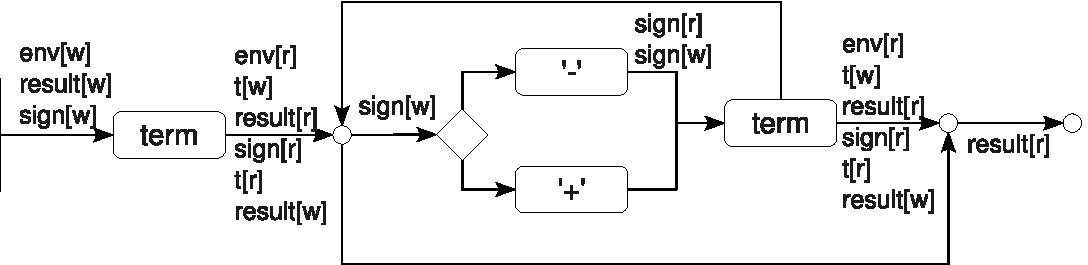
\includegraphics[width=\textwidth]{cfg.pdf}
	\caption{Граф потока управления для правила \texttt{expr}, помеченный обращениями к атрибутам}\label{cfg}
\end{figure}

\chapter{Контроль типов в семантических действиях}

Как отмечалось выше, проверка типов в семантических действиях позволяет обнаруживать ошибки в спецификации и не допускать их появления в сгенерированном коде. В данном разделе мы опишем систему типов языка \ATF{} и приведем примеры ее использования.

\section{Правила системы типов}

\renewcommand{\L}{{}}
\newcommand{\G}{ {\mathcal{G}_\L} }
\newcommand{\eql}{\cong_\L}
\newcommand{\lel}{\preceq_\L}
\newcommand{\gel}{\succeq_\L}
\newcommand{\TUP}{TupleType}
\newcommand{\Str}{String_\L}

Правила системы типов \ATF{} содержат следующие параметры, уточняющиеся для каждой спецификации:
\begin{itemize}
\item множество \term{базовых типов} $\G$ (от \emph{ground});
\item выделенный \term{строковый тип} $\Str \in \G$;
\item транзитивное рефлексивное отношение $\lel \;\subseteq \G \times \G$ (и $\gel \;:=\; \lel^{\top}$), где 
	\begin{itemize}
	\item ``$\tau \lel \sigma$''
читается как ``$\tau$ является \term{подтипом} $\sigma$'', а
	\item ``$\tau \gel \sigma$''
читается как ``$\tau$ является \term{супертипом} $\sigma$''.
	\end{itemize}
\end{itemize}

Язык типов \ATF{} описывается следующими продукциями:
$$
\begin{array}{rcll}
	AttributeType &::=& \G              &\mbox{--- тип атрибута}\\
	TupleType &::=& (AttributeType^*)   &\mbox{--- тип кортежа}\\
	FunctionType &::=& 
	   TupleType \rightarrow TupleType  &\mbox{--- тип функции}\\
\end{array}
$$
Таким образом, атрибуты могут иметь только базовые типы, а функции принимают на вход и возвращают кортежи. Заметим, что кортеж может иметь ноль или более компонент.

Корректность типов проверяется отдельно в каждой функции трансляции. \term{Контекст} $\Gamma$ является множеством деклараций всех функций, объявленных в спецификации, а также всех входных и выходных атрибутов этих функций и локальных атрибутов той функции, которая проверяется в данный момент. Поскольку атрибуты в разных функциях могут иметь одинаковые имена, мы выносим имя функции в верхний индекс имени атрибута. Например, контекст может содержать следующий набор деклараций:
$$\begin{array}{rcl}
factor&:& (Environment) \rightarrow (Int)\\
env^{factor} &:& Environment\\
result^{factor} &:& Int\\
term &:& (Environment) \rightarrow (Int)\\
env^{term} &:& Environment\\
result^{term} &:& Int\\
\end{array}$$

На \figref{exptypes} приведены очевидные правила типизации для атрибутов, токенов и кортежей, а также правило для функций, говорящее, что тип фактического аргумента должен являться подтипом типа формального параметра.
\begin{figure}[htbp]
$$\begin{array}{lll}

	\begin{array}{l}
		\trule{}{\Gamma \vdash \mathtt{NAME\#} : \Str}{token}\\
		\\
		\trule{}{\Gamma, \alpha : \tau \vdash \alpha : \tau }{attribute}\\
	\end{array}
&&
\trule{
\begin{array}{l}
	\tau_1 \ldots\tau_n \in \G\\
	\Gamma \vdash x_1 : \tau_1 \, \ldots \, \Gamma \vdash x_n : \tau_n
\end{array}
}{
	\Gamma \vdash (x_1, \ldots, x_n) : (\tau_1, \ldots, \tau_n)
}{tuple}

\\
&&\hspace{10pt}\\
\multicolumn{3}{c}{
\trule{	
\begin{array}{lll}
		\tau_1 \ldots\tau_n,\, \sigma_1 \ldots \sigma_n,\, \rho_1 \ldots \rho_m \in \G
		&\quad&
		\sigma_1 \gel \rho_1\,\ldots\, \sigma_m \gel \rho_m\\
		\Gamma \vdash f : (\sigma_1,\,\ldots,\,\sigma_m) \rightarrow (\tau_1,\,\ldots,\,\tau_n)
		&\quad&
		\Gamma \vdash x_1 : \rho_1 \, \ldots \, \Gamma \vdash x_n : \rho_n\\
\end{array}
}{\Gamma \vdash f(x_1,\,\ldots,\,x_m) : (\tau_1,\,\ldots,\,\tau_n)}{app}
}
\end{array}$$
\caption{Базовые правила для выражений \ATF{}}\label{exptypes}
\end{figure}
На \figref{statypes} приведены правила типизации, контролирующие структуру правильных предложений \ATF{}, контролирующие типизацию в присваиваниях и вызовах функций, результат которых не используется. 
\begin{figure}[htbp]
$$
\begin{array}{l}
\trule{
\begin{array}{l}
\sigma,\,\tau \in \G \cup \TUP
\\
\Gamma \vdash \alpha : \sigma 
\quad 
\Gamma \vdash \beta : \tau 
\quad 
\sigma \gel^* \tau
\end{array}
}{\Gamma \vdash \alpha = \beta \in CorrectStatement}{assignment}
\vspace{10pt}
\\
\trule{
\Gamma \vdash f(x_1,\,\ldots,\,x_m) : \rho
}{
\Gamma \vdash f(x_1,\,\ldots,\,x_m) \in CorrectStatement
}{app-statement}
\vspace{10pt}
\\
\trule{
\Gamma \vdash \alpha_1,\,\ldots,\,\alpha_n \in CorrectStatement
}{\Gamma \vdash \left\{ \alpha_1,\,\ldots,\,\alpha_n \right\} \in CorrectStatement}{block}
\end{array}
$$
\caption{Базовые правила для предложений \ATF{}}\label{statypes}
\end{figure}
Множество $CorrectStatement$ обозначает все предложения, удовлетворяющие требованиям системы типов. Поскольку результатом функции, а также значением слева от знака равенства может быть кортеж, правило для присваивания (assignment) использует отношение $\gel^*$, являющееся покомпонентным расширением $\gel$ на кортежи:
$$(a_1,\cdots,a_n)\gel^*(b_1,\cdots,b_n)
	\;\Leftrightarrow\; 
(a_1 \gel b_1) \wedge \cdots \wedge (a_n \gel b_n)$$

\section{Локальный вывод типов}

Система типов \ATF{} позволяет во многих случаях не декларировать локальные атрибуты и внешние функции, поскольку информация об их типах может быть автоматических реконструирована из контекста. 

Типы реконструируются отдельно внутри каждой функции трансляции. Любой атрибут, не имеющий объявления, считается локальным, а любая не объявленная, но использованная функция -- внешней. При этом, зная типы входных и выходных атрибутов функций трансляции, которые декларировать обязательно, можно составить ``неравенства'' для типов атрибутов, решая которые можно определить эти типы.
Для этого тело функции трансляции представляется в виде множества присваиваний атрибутов. Вызовы функций представляются как набор присваиваний аргументов формальным параметрам, а результаты функций представляются их выходными атрибутами. 

Приведем простой пример, основанный на приведенном выше правиле для символа \code{expr}, в котором не объявлен, но использован атрибут \code{t}. Соответствующая функция трансляции содержит следующие строки:
\begin{lstlisting}[language=Grammatic]
	at     term : t = term(env);
	after  term : result = add(result, mul(sign, t));
\end{lstlisting}
Напомним, что функция трансляции \code{term} и внешняя функция \code{mul} имеют следующие сигнатуры:
\begin{lstlisting}[language=Grammatic]
	mul(x : Int, y : Int) -> (prod : Int);
	term(env : Environment) -> (result : Int);
\end{lstlisting}
Для атрибута \code{t}, действие в функции \code{expr} представляется в виде двух присваиваний. Сначала ему присваивается выходной атрибут функции \code{term}:
\begin{equation}\label{teqres}
		t \leftarrow result^{term} : \mathtt{Int}
\end{equation}
Затем сам \code{t} присваивается входному атрибуту \code{y} функции \code{mul}:
\begin{equation}\label{yeqt}
		y^{mul} : \mathtt{Int} \leftarrow t
\end{equation}
На основе этих двух присваиваний и правил на \figref{exptypes} можно составить следующую систему ограничений для переменной $\tau$, обозначающей неизвестный тип атрибута \code{t}:
$$
	\left\{\begin{array}{l}%
		\tau \lel \mathtt{Int}\\
		\mathtt{Int} \lel \tau\\
	\end{array}\right.
$$
Решение этой системы очевидно: $\tau = \mathtt{Int}$.

В общем случае для реконструкции используется модификация стандартного алгоритма, описанного, например в \cite{Pierce}. Мы не будем повторять описание этого алгоритма, а лишь опишем поведение нашей модификации в случае неоднозначности. Предположим, что $\G = \{Object, Integer\}$, причем $Integer \lel Object$, и рассмотрим следующую функцию трансляции:
\begin{lstlisting}[language=Grammatic]
f(x : Integer) -> (result : Object) {
	before ... : t = x;
	// ...
	after  ... : result = t;
}
\end{lstlisting}
Локальный атрибут \code{t} не объявлен. Пусть $\tau$ обозначает неизвестный тип этого атрибута. Алгоритм реконструкции типов построит следующую систему ограничений:
$$\left.\begin{array}{l}
Integer \lel \tau\\
\tau \gel Object\\
\end{array}\right\}$$
Эта система имеет два решения: и $Object$, и $Integer$ удовлетворяют обоим ограничениям. Существование решения уже означает, что спецификация не содержит ошибок типизации, но, как мы увидим ниже модулю генерации нужен некоторый тип, чтобы сгенерировать код, поэтому необходимо выбрать одно из решений.
Конкретные значения типовых переменных важны при генерации сигнатур внешних функций на языке реализации, которые видит разработчик, поэтому выбирать типы произвольно нельзя.

В таких ситуациях \ATF{} предпочитает нижние границы верхним, что в данном случае означает, что будет выбран тип $Integer$. В общем случае процедура выглядит следующим образом: выбирается минимальное решение, удовлетворяющее всем ограничениям снизу, если оно удовлетворяет также всем ограничениям сверху, выбрать это решение. Если существует несколько несравнимых решений, удовлетворяющих всем ограничениям снизу, алгоритм не может выбрать из них одно и выдает сообщение об ошибке. Если нет ни одного такого решения, значит система противоречива и в этом случае тоже генерируется сообщение об ошибке. Если в системе нет ни одного ограничения снизу, выбирается \emph{максимальное} решение, удовлетворяющее всем ограничениям сверху.

Эту процедуру можно обобщить следующим образом: производится поиск решения как можно более близкого к ограничивающим типам, причем предпочтение отдается более конкретным (меньшим) типам. Опыт использования \ATF{} показывает, что этот метода как правило дает результаты, соответствующие интуиции разработчика.

Возможна ситуация, когда в системе не упоминается ни одного базового типа. Это означает, что все атрибуты, связанные с данным, не объявлены. В этом случае \ATF{} проверяет, существует ли в системе наибольший тип $Top_\L$, для которого выполняется $\tau \lel Top_\L$ при любом $\tau$. Если такой тип существует, он выбирается в качестве решения. Если нет --- генерируется сообщение об ошибке.

\section{Пример работы механизма проверки типов}
Вернемся к примеру, приведенному в разделе \ref{antlr_example} и покажем, как система типов \ATF{} облегчает работу программиста в этой ситуации. Мы рассматривали правило для символа \code{factor}, в котором была допущена ошибка: вместо текстового значения токена \code{INT} был использован сам объект токена. В следующей функции трансляции допущена такая же ошибка:
\begin{lstlisting}
factor : VAR | INT | '(' expr ')' ;          
	factor(Environment env) --> (Int result) { 
		after VAR : result = evaluate(env, VAR#);  
		after INT : result = INT;
		at expr   : result = expr(env);           
	}
\end{lstlisting}
В отличие от \tool{ANTLR}, \ATF{} генерирует сообщение об ошибке при попытке сгенерировать код по данной спецификации, а не после компиляции сгенерированного кода. Поясним, как это происходит: имя \code{INT} нигде не объявлено \footnote{Использовать символы грамматики непосредственно в семантических действиях \ATF{} не позволяет}, поэтому оно рассматривается рассматривается как имя локального атрибута, который присваивается выходному атрибуту \code{result}, но нигде не инициализируется. Генерируется сообщение об ошибке с строке.

Не генерируя код и не запуская компилятор, мы получили сообщение об ошибке, указывающее на строку в спецификации, являющуюся его причиной. Проблема в том, что мы использовали имя токена там, где должны были использовать операцию \code{\#} для того, чтобы получить его текстовое значение. Мы вносим исправление:
\begin{lstlisting}
	after INT : result = INT#;
\end{lstlisting}
При попытке сгенерировать код мы получаем следующее сообщение об ошибке: типы \texttt{String} и \texttt{Int} не совместимы. Мы должны преобразовать строку в число для того, чтобы выполнить присваивание:
\begin{lstlisting}
	after INT : result = strToInt(INT#);
\end{lstlisting}
На этот раз генерация кода проходит успешно и сгенерированный код не содержит ошибок.

Мы убедились в том, что цикл разработки при использовании \ATF{} соответствует \figref{cycles} (б), то есть мы достигли одной из двух поставленных целей. Ниже мы опишем, каким образом этот механизм работает для нескольких языков реализации одновременно.

\section{Способы описания базовых типов}

Правила, описанные в предыдущих разделах, параметризованы следующими понятиями, в совокупности определяющими \term{систему типов абстрактного уровня}:
\begin{itemize}
\item множество \term{базовых типов} $\G$ (от \emph{ground});
\item выделенный \term{строковый тип} $\Str \in \G$;
\item отношение $\lel \;\subseteq \G \times \G$.
\end{itemize}
Для проверки типов в конкретной спецификации необходимо придать смысл этим понятиям. Дополнительно, для того, чтобы сгенерировать код, необходимо отображение из множества $\G$ в множество типов языка реализации.
Для решения этой задачи \ATF{} предоставляет механизм \term{расширений}, позволяющий встраивать в общий механизм проверки и вывода типов модули, придающие значения параметрам. 

В следующих разделах мы опишем стандартное расширение, используемое по умолчанию, позволяющее декларативно описывать системы типов абстрактного уровня, а также расширение для тесной интеграции с системой типов \tool{Java}.

\subsection{Декларативное описание системы типов}

Множество базовых типов $\G$ и отношение $\lel$ декларативно задаются прямым перечислением в конструкции \code{typesystem} как показано в \lstref{typesystem}. 
\begin{lstlisting}[language=Typesystem,label=typesystem,float=htbp,
caption=Декларативное описание типов абстрактного уровня]
typesystem Simple( 
	_,             // Наибольший тип (отсутствует в данном случае)
	String         // Строковый тип
) {
	// Объявления типов (множество $\G$)
	type Int;
	type Environment;
	type Object;
	type String;

	// Отношение $\lel$
	Environment <: Object;
	String      <: Object;
}
\end{lstlisting}
За ключевым словом \code{typesystem} следует имя системы типов, далее в скобках указывается выделенный тип $\Str$. Далее следуют описания типов и неравенства. Отношение $\lel$ строится как рефлексивное транзитивное замыкание отношения, данного в декларативном описании системы типов.

Такой спецификации достаточно, чтобы проверить и реконструировать типы в спецификации на языке \ATF{}. Для того, чтобы сгенерировать код, необходимо указать, какие типы языка реализации (далее мы будем называть их \term{типами конкретного уровня}) сопоставляются типам абстрактного уровня. Это также описывается декларативно с помощью конструкции \code{language}. 
\begin{lstlisting}[language=Typesystem,label=language,float=htbp,
caption=Декларативное описание типов конкретного уровня]
language Java for Simple {
	Int = 'int';
	Environment = 'java.util.Map<String, Integer>';
	String = 'String';
	Object = 'Object';
}
\end{lstlisting}
В  \lstref{language} показано такое описание для языка \tool{Java}: типам абстрактного уровня сопоставляются строки, которые будут использованы модулем генерации. Если проверки в модуле анализа прошли успешно и типы конкретного уровня удовлетворяют отношению $\lel$ для соответствующих типов абстрактного уровня, сгенерированный код не будет содержать ошибок типизации.

\subsection{Механизм расширений}

Архитектура \ATF{} позволяет подключать различные расширения, вводящие другие способы описания базовых типов. В качестве примера рассмотрим расширение, позволяющее использовать типы языка \tool{Java} в спецификациях \ATF{} непосредственно, без описания абстрактного уровня.

Данное расширение задает синтаксическую форму языка типов в соответствии с правилами языка \tool{Java}, вводит инструкцию \code{javaimport} для импортирования классов и осуществляет поиск типов аналогично тому как это делает компилятор \tool{Java}. В результате, например, описание внешней функции может выглядеть так:
\begin{lstlisting}[language=Java]
import java.util.Map;

evaluate(environment : Map<String, Integer>) -> (result : Integer);
\end{lstlisting}
Аналогично типы могут быть использованы и в других частях спецификации.

Такое расширение, очевидно, не допускает генерации кода на языках, не совместимых в \tool{Java}, однако оно может быть полезно, если данная функциональность не требуется, а более тесная интеграция с языком реализации упрощает работу с \ATF{}.

\subsection{Генерируемые артефакты}

\chapter{Реализация на основе \GRM{}}

\chapter{Применение предложенного подхода}

Grammatic на Java

\chapter{Выводы}